\documentclass[aspectratio=169]{beamer}

% ── REQUIRED PACKAGES ─────────────────────────────────────────────
\usetheme{metropolis}
\usepackage{tikz}
\usepackage{tcolorbox}
\usepackage{fontawesome5}
\usepackage{minted}
\usepackage{pgfplots}
\usepackage{graphicx}
\usepackage{xcolor}
\usepackage{booktabs}
\usepackage{array}
\usepackage{hyperref}
\usepackage{animate}
\usepackage{lmodern}

\usetikzlibrary{arrows.meta, shapes, positioning, fit, backgrounds, shadows, calc, decorations.pathreplacing}
\tcbuselibrary{skins, breakable, listings}
\pgfplotsset{compat=1.18}

% ── CUSTOM COLOR PALETTE ──────────────────────────────────────────
\definecolor{primary}{HTML}{0F172A}     % Deep navy
\definecolor{accent}{HTML}{38BDF8}      % Electric blue
\definecolor{accentsec}{HTML}{818CF8}   % Indigo
\definecolor{success}{HTML}{34D399}     % Emerald
\definecolor{warning}{HTML}{FBBF24}     % Amber
\definecolor{bgbody}{HTML}{1E293B}      % Slate dark
\definecolor{surface}{HTML}{0F172A}     % Darker navy
\definecolor{textprim}{HTML}{F1F5F9}    % Near white
\definecolor{textsec}{HTML}{94A3B8}     % Slate gray

\definecolor{cMongo}{HTML}{14B8A6}      % Teal
\definecolor{cDebezium}{HTML}{A855F7}   % Purple
\definecolor{cKafka}{HTML}{F59E0B}      % Amber
\definecolor{cElastic}{HTML}{F43F5E}    % Coral

% ── THEME OVERRIDES ───────────────────────────────────────────────
\setbeamercolor{normal text}{fg=textprim, bg=bgbody}
\setbeamercolor{frametitle}{bg=primary, fg=white}
\setbeamercolor{progress bar}{fg=accent, bg=surface}
\setbeamercolor{alerted text}{fg=accent}
\setbeamercolor{itemize item}{fg=accent}
\setbeamercolor{itemize subitem}{fg=accentsec}

\setbeamerfont{frametitle}{size=\Large, series=\bfseries}
\setbeamerfont{title}{size=\huge, series=\bfseries}
\setbeamerfont{subtitle}{size=\Large, series=\mdseries}

% Add thin horizontal accent line under frametitle
\addtobeamertemplate{frametitle}{}{%
  \begin{tikzpicture}[remember picture,overlay]
    \draw[accent, thick] (current page.north west) ++(0,-1.02) -- ++(\paperwidth,0);
  \end{tikzpicture}
}

% ── CUSTOM STYLES & MACROS ────────────────────────────────────────
\tikzset{
    component/.style={
        rectangle, rounded corners, draw=surface, fill=surface, 
        thick, text=white, align=center, minimum width=2.8cm, minimum height=1.5cm,
        drop shadow={opacity=0.2}
    },
    arrow/.style={
        -{Stealth[length=3mm]}, thick, draw=accent
    },
    stepcircle/.style={
        circle, fill=accent, text=primary, font=\bfseries, 
        minimum size=0.6cm, inner sep=0pt
    }
}

\tcbset{
    card/.style={
        enhanced, colback=surface, colframe=surface, arc=4mm, 
        boxrule=0pt, drop shadow={opacity=0.2}, coltext=textprim
    },
    badcard/.style={card, colback=red!10!bgbody, colframe=red!30!bgbody, boxrule=1pt},
    goodcard/.style={card, colback=green!10!bgbody, colframe=green!30!bgbody, boxrule=1pt},
    codebox/.style={card, colback=primary, arc=2mm, top=0pt, bottom=0pt, left=0pt, right=0pt}
}

\setminted{
    style=monokai,
    fontsize=\scriptsize,
    bgcolor=primary,
    linenos=false,
    tabsize=2
}

% Image placeholder macro
% Usage: \imageplaceholder{filename}{width}{placeholder height}
\newcommand{\imageplaceholder}[3]{%
  \begin{figure}
  \IfFileExists{images/#1}{%
    \includegraphics[width=#2]{images/#1}%
  }{%
    \fbox{\begin{tikzpicture}
      \node[fill=surface, text=textsec, minimum width=#2, minimum height=#3, align=center] {
        \faImage\\[1ex] \small [IMAGE: #1]
      };
    \end{tikzpicture}}
  }
  \end{figure}
}

% ── DOCUMENT INFO ─────────────────────────────────────────────────
\title{\textcolor{accent}{Real-Time Data Synchronization} with CDC}
\subtitle{\textcolor{accentsec}{MongoDB \faAngleRight\ Debezium \faAngleRight\ Kafka \faAngleRight\ Elasticsearch}}
\author{[AUTHOR NAME]}
\date{\today}
\institute{[CONFERENCE / COURSE NAME]}

\begin{document}

% ==================================================================
% SLIDE 1: TITLE SLIDE
% ==================================================================
{
\setbeamertemplate{footline}{} % Hide progress bar on title slide
\begin{frame}[plain]
  \begin{tikzpicture}[remember picture, overlay]
    % Background
    \fill[primary] (current page.south west) rectangle (current page.north east);
    
    % Subtle dot grid background
    \begin{scope}[opacity=0.1]
      \foreach \x in {0,1,...,16} {
        \foreach \y in {0,1,...,9} {
          \fill[textsec] (\x,\y) circle (1pt);
        }
      }
    \end{scope}

    % Logo Placeholder
    \node[anchor=north west, inner sep=15pt] at (current page.north west) {
      \IfFileExists{images/logo.png}{
        \includegraphics[width=2cm]{images/logo.png}
      }{
        \color{textsec}\faCode\ \small [LOGO]
      }
    };

    % Title and Subtitle
    \node[anchor=center, align=center] at ($(current page.center)+(0,1.5)$) {
      {\Huge\bfseries\color{white} Real-Time Data Synchronization \textcolor{accent}{with CDC}}\\[0.5em]
      {\Large\color{accentsec} MongoDB \faAngleRight\ Debezium \faAngleRight\ Kafka \faAngleRight\ Elasticsearch}
    };

    % Horizontal Pipeline Diagram
    \node[anchor=center] at ($(current page.center)+(0,-1)$) {
      \begin{tikzpicture}
        \node[component, fill=cMongo!20!surface, draw=cMongo] (mongo) {\faDatabase\\[0.5em] MongoDB};
        \node[component, fill=cDebezium!20!surface, draw=cDebezium, right=1.5cm of mongo] (debezium) {\faPlug\\[0.5em] Debezium};
        \node[component, fill=cKafka!20!surface, draw=cKafka, right=1.5cm of debezium] (kafka) {\faStream\\[0.5em] Kafka};
        \node[component, fill=cElastic!20!surface, draw=cElastic, right=1.5cm of kafka] (elastic) {\faSearch\\[0.5em] Elastic};
        
        \draw[arrow, cMongo] (mongo) -- (debezium);
        \draw[arrow, cDebezium] (debezium) -- (kafka);
        \draw[arrow, cKafka] (kafka) -- (elastic);
      \end{tikzpicture}
    };

    % Author and Date
    \node[anchor=south west, inner sep=15pt] at (current page.south west) {
      \color{textsec}\small [AUTHOR NAME] \quad|\quad [CONFERENCE / COURSE NAME]
    };
    \node[anchor=south east, inner sep=15pt] at (current page.south east) {
      \color{textsec}\small \today
    };
  \end{tikzpicture}
\end{frame}
}

% ==================================================================
% SLIDE 2: TABLE OF CONTENTS
% ==================================================================
\begin{frame}{Agenda}
  \vspace{0.5cm}
  
\begin{tikzpicture}[node distance=0.8cm and 0.5cm]
    \node[stepcircle] (n1) {1};
    \node[right=of n1, font=\Large\color{white}, yshift=-1pt] (t1) {The Problem \& Solution};
    \draw[textsec!30, thin] ($(t1.south west)+(0,-0.1)$) -- ($(t1.south east)+(5,-0.1)$);
    
    \node[stepcircle, below=of n1] (n2) {2};
    \node[right=of n2, font=\Large\color{white}, yshift=-1pt] (t2) {System Architecture};
    \draw[textsec!30, thin] ($(t2.south west)+(0,-0.1)$) -- ($(t2.south east)+(5,-0.1)$);

    \node[stepcircle, below=of n2] (n3) {3};
    \node[right=of n3, font=\Large\color{white}, yshift=-1pt] (t3) {Component Deep Dive};
    \draw[textsec!30, thin] ($(t3.south west)+(0,-0.1)$) -- ($(t3.south east)+(5,-0.1)$);

    \node[stepcircle, below=of n3] (n4) {4};
    \node[right=of n4, font=\Large\color{white}, yshift=-1pt] (t4) {Live Pipeline Demo};
    \draw[textsec!30, thin] ($(t4.south west)+(0,-0.1)$) -- ($(t4.south east)+(5,-0.1)$);

    \node[stepcircle, below=of n4] (n5) {5};
    \node[right=of n5, font=\Large\color{white}, yshift=-1pt] (t5) {Results \& Observability};
    \draw[textsec!30, thin] ($(t5.south west)+(0,-0.1)$) -- ($(t5.south east)+(5,-0.1)$);
  \end{tikzpicture}
\end{frame}

% ==================================================================
% SLIDE 3: THE PROBLEM WE SOLVE
% ==================================================================
\begin{frame}{The Problem We Solve}
  \begin{columns}[T]
    \begin{column}{0.48\textwidth}
      \begin{tcolorbox}[badcard, title=\faTimesCircle\ Without CDC (Batch)]
        \begin{itemize}
            \item Batch jobs run every hour \faArrowRight\ stale search results
            \item Manual sync scripts \faArrowRight\ brittle and error-prone
            \item Downtime required for bulk re-indexing
            \item No audit trail of what changed and when
        \end{itemize}
      \end{tcolorbox}
    \end{column}
    \begin{column}{0.48\textwidth}
      \begin{tcolorbox}[goodcard, title=\faCheckCircle\ With CDC (Real-Time)]
        \begin{itemize}
            \item Sub-200ms latency from write to search
            \item Zero application code changes needed
            \item Full audit log of every atomic change
            \item Fault-tolerant: survives restarts safely
        \end{itemize}
      \end{tcolorbox}
    \end{column}
  \end{columns}
  
  \vspace{0.3cm}
  % PLACEHOLDER: replace with actual screenshot
  \imageplaceholder{problem-diagram.png}{0.5\textwidth}{2.5cm}
  \vspace{-0.3cm}
  \begin{center}\scriptsize\color{textsec} Traditional batch sync vs real-time CDC\end{center}
\end{frame}

% ==================================================================
% SLIDE 4: SECTION DIVIDER 1
% ==================================================================
\begin{frame}[plain]
  \begin{tikzpicture}[remember picture, overlay]
    \fill[bgbody] (current page.south west) rectangle (current page.north east);
    
    % Left accent panel
    \fill[accent] (current page.south west) rectangle ([xshift=0.33\paperwidth]current page.north west);
    
    % Decorative pattern
    \begin{scope}[opacity=0.2]
      \draw[white, thick] (-1,0) -- (4,5);
      \draw[white, thick] (-1,2) -- (4,7);
      \draw[white, thick] (-1,4) -- (4,9);
    \end{scope}

    \node[anchor=center, text=primary, font=\fontsize{60}{60}\bfseries] at ([xshift=0.165\paperwidth]current page.center) {01};
    
    \node[anchor=west, text=white] at ([xshift=0.38\paperwidth]current page.west) {
      \begin{minipage}{0.55\textwidth}
        {\Huge\bfseries System Architecture}\\[0.5em]
        {\Large\color{accentsec} Designing the data flow from source to search.}
      \end{minipage}
    };
  \end{tikzpicture}
\end{frame}

% ==================================================================
% SLIDE 5: PIPELINE ARCHITECTURE
% ==================================================================
\begin{frame}{Complete Pipeline Architecture}
  \begin{center}
    
\begin{tikzpicture}[node distance=1.8cm, every node/.style={scale=0.9}]
      % Nodes
      \node[component, fill=cMongo!10!surface, draw=cMongo] (mongo) {
        \textcolor{cMongo}{\faDatabase}\\[0.3em]
        \textbf{MongoDB}\\[0.1em]
        \scriptsize Source Database
      };
      
      \node[component, fill=cDebezium!10!surface, draw=cDebezium, right=of mongo] (connect) {
        \textcolor{cDebezium}{\faPlug}\\[0.3em]
        \textbf{Kafka Connect}\\[0.1em]
        \scriptsize Debezium + ES Sink
      };

      \node[component, fill=cKafka!10!surface, draw=cKafka, right=of connect] (kafka) {
        \textcolor{cKafka}{\faStream}\\[0.3em]
        \textbf{Apache Kafka}\\[0.1em]
        \scriptsize Event Broker
      };

      \node[component, fill=cElastic!10!surface, draw=cElastic, right=of kafka] (elastic) {
        \textcolor{cElastic}{\faSearch}\\[0.3em]
        \textbf{Elasticsearch}\\[0.1em]
        \scriptsize Search Engine
      };

      % Ports
      \node[below=0.2cm of mongo, text=textsec, font=\tiny] {Port 27017};
      \node[below=0.2cm of connect, text=textsec, font=\tiny] {Port 8083};
      \node[below=0.2cm of kafka, text=textsec, font=\tiny] {Port 9092};
      \node[below=0.2cm of elastic, text=textsec, font=\tiny] {Port 9200};

      % Arrows
      \draw[arrow, cMongo] (mongo) -- node[above, font=\scriptsize, text=white] {oplog} (connect);
      \draw[arrow, cDebezium] ([yshift=0.2cm]connect.east) -- node[above, font=\scriptsize, text=white] {produce} ([yshift=0.2cm]kafka.west);
      \draw[arrow, cElastic] ([yshift=-0.2cm]kafka.west) -- node[below, font=\scriptsize, text=white] {consume} ([yshift=-0.2cm]connect.east);
      \draw[arrow, cKafka] (connect) -- node[above, font=\scriptsize, text=white] {upsert} (elastic);
    \end{tikzpicture}
  \end{center}
  
  \vspace{0.3cm}
  % PLACEHOLDER: replace with actual screenshot
  \imageplaceholder{architecture-screenshot.png}{0.8\textwidth}{2.5cm}
  \vspace{-0.3cm}
  \begin{center}\scriptsize\color{textsec} Live pipeline running natively in Docker\end{center}
\end{frame}

% ==================================================================
% SLIDE 6: DOCKER INFRASTRUCTURE
% ==================================================================
\begin{frame}[fragile]{Docker Infrastructure}
  \begin{columns}[T]
    \begin{column}{0.35\textwidth}
      \begin{tcolorbox}[card, title=\faFolderOpen\ Project Structure]
        \ttfamily\scriptsize
        \textcolor{accent}{\faFolderOpen\ cdc-pipeline/}\\
        \hspace*{0.5cm}\textcolor{textsec}{\faFolder\ app/}\\
        \hspace*{1.0cm}\faFileCode\ demo.py\\
        \hspace*{0.5cm}\textcolor{textsec}{\faFolder\ connectors/}\\
        \hspace*{1.0cm}\faFileCode\ mongodb-source.json\\
        \hspace*{1.0cm}\faFileCode\ elastic-sink.json\\
        \hspace*{0.5cm}\textcolor{textsec}{\faFolder\ scripts/}\\
        \hspace*{1.0cm}\faTerminal\ init-mongo.js\\
        \hspace*{1.0cm}\faTerminal\ test-pipeline.sh\\
        \hspace*{0.5cm}\textcolor{success}{\faDocker\ docker-compose.yml}
      \end{tcolorbox}
    \end{column}
    \begin{column}{0.6\textwidth}
      \begin{tcolorbox}[codebox]
\begin{minted}{yaml}
kafka:
  image: apache/kafka:3.7.0
  environment:
    KAFKA_NODE_ID: 1
    KAFKA_PROCESS_ROLES: broker,controller
    KAFKA_LISTENERS: PLAINTEXT://:9092,CONTROLLER://:9093
    KAFKA_CONTROLLER_LISTENER_NAMES: CONTROLLER
    KAFKA_CONTROLLER_QUORUM_VOTERS: 1@localhost:9093
\end{minted}
      \end{tcolorbox}
      
\begin{tikzpicture}[overlay, remember picture]
        \node[fill=accentsec, text=white, rounded corners, inner sep=4pt, font=\scriptsize, drop shadow] 
          (callout) at (0, 0.5) {\faInfoCircle\ No Zookeeper needed!};
        \draw[accentsec, thick, -{Stealth}] (callout.north) ++(2,0) -- ++(1, 1.5);
      \end{tikzpicture}
    \end{column}
  \end{columns}
  
  \vspace{0.4cm}
  % PLACEHOLDER: replace with actual screenshot
  \imageplaceholder{docker-dashboard.png}{0.45\textwidth}{2cm}
  \vspace{-0.3cm}
  \begin{center}\scriptsize\color{textsec} All 6 services running cleanly\end{center}
\end{frame}

% ==================================================================
% SLIDE 7: SECTION DIVIDER 2
% ==================================================================
\begin{frame}[plain]
  \begin{tikzpicture}[remember picture, overlay]
    \fill[bgbody] (current page.south west) rectangle (current page.north east);
    \fill[accent] (current page.south west) rectangle ([xshift=0.33\paperwidth]current page.north west);
    
    \begin{scope}[opacity=0.2]
      \draw[white, thick] (-1,0) -- (4,5);
      \draw[white, thick] (-1,2) -- (4,7);
      \draw[white, thick] (-1,4) -- (4,9);
    \end{scope}

    \node[anchor=center, text=primary, font=\fontsize{60}{60}\bfseries] at ([xshift=0.165\paperwidth]current page.center) {02};
    
    \node[anchor=west, text=white] at ([xshift=0.38\paperwidth]current page.west) {
      \begin{minipage}{0.55\textwidth}
        {\Huge\bfseries Component Deep Dive}\\[0.5em]
        {\Large\color{accentsec} Understanding the engine under the hood.}
      \end{minipage}
    };
  \end{tikzpicture}
\end{frame}

% ==================================================================
% SLIDE 8: MONGODB & THE OPLOG
% ==================================================================
\begin{frame}[fragile]{MongoDB \& The Oplog}
  \begin{columns}[T]
    \begin{column}{0.31\textwidth}
      \begin{tcolorbox}[card, title=\faServer\ Replica Set]
        \scriptsize Debezium requires a MongoDB replica set (\texttt{rs0}). A standalone MongoDB does not generate an oplog.
      \end{tcolorbox}
    \end{column}
    \begin{column}{0.31\textwidth}
      \begin{tcolorbox}[card, title=\faBook\ The Oplog]
        \scriptsize A capped collection that keeps a rolling record of all operations that modify the database's data.
      \end{tcolorbox}
    \end{column}
    \begin{column}{0.31\textwidth}
      \begin{tcolorbox}[card, title=\faLayerGroup\ Collections]
        \scriptsize We stream changes from \texttt{users}, \texttt{products}, and \texttt{orders} in the \texttt{appdb} database.
      \end{tcolorbox}
    \end{column}
  \end{columns}

  \vspace{0.4cm}
  \textbf{\color{accent} Raw Oplog Entry Format:}
  \begin{tcolorbox}[codebox]
\begin{minted}{javascript}
{ 
  "ts": Timestamp(1623456789, 1), 
  "op": "i", 
  "ns": "appdb.users", 
  "o": { "_id": ObjectId("..."), "name": "Alice", "role": "engineer" } 
}
\end{minted}
  \end{tcolorbox}

  \vspace{0.2cm}
  % PLACEHOLDER: replace with actual screenshot
  \imageplaceholder{mongo-compass.png}{0.55\textwidth}{2cm}
  \vspace{-0.3cm}
  \begin{center}\scriptsize\color{textsec} MongoDB Compass showing the oplog\end{center}
\end{frame}

% ==================================================================
% SLIDE 9: DEBEZIUM: THE CDC ENGINE
% ==================================================================
\begin{frame}[fragile]{Debezium: The CDC Engine}
  \begin{columns}[T]
    \begin{column}{0.4\textwidth}
      \vspace{0.5cm}
      \textcolor{accent}{\Huge \faBroadcastTower}
      \vspace{0.5cm}
      \begin{itemize}
        \item Acts as a MongoDB replica
        \item Tails the oplog in real-time
        \item \textbf{Snapshot Mode:} Dumps existing data on first boot
        \item \textbf{SMT (Single Message Transforms):} Cleans complex payloads before sending to Kafka
      \end{itemize}
    \end{column}
    
    \begin{column}{0.55\textwidth}
      \begin{tcolorbox}[codebox]
\begin{minted}{json}
{
  "name": "mongodb-source",
  "config": {
    "connector.class": "io.debezium...MongoDbConnector",
    "mongodb.connection.string": "mongodb://mongodb/?replicaSet=rs0",
    "database.include.list": "appdb",
    "topic.prefix": "dbserver1",
    "capture.mode": "change_streams_update_full",
    "transforms": "unwrap",
    "transforms.unwrap.type": "...ExtractNewDocumentState",
    "transforms.unwrap.drop.tombstones": "false",
    "transforms.unwrap.delete.handling.mode": "rewrite"
  }
}
\end{minted}
      \end{tcolorbox}
    \end{column}
  \end{columns}

  \vspace{0.2cm}
  % PLACEHOLDER: replace with actual screenshot
  \imageplaceholder{debezium-ui.png}{0.45\textwidth}{1.5cm}
  \vspace{-0.3cm}
  \begin{center}\scriptsize\color{textsec} Debezium connector status: RUNNING\end{center}
\end{frame}

% ==================================================================
% SLIDE 10: THE CDC EVENT FORMAT
% ==================================================================
\begin{frame}[fragile]{The CDC Event Format}
  \begin{columns}[T]
    \begin{column}{0.7\textwidth}
      \begin{tcolorbox}[codebox]
\begin{minted}{json}
{
  "_id": "6a3bdb4cc0bf539cca9df8a3",
  "name": "Alice Johnson",
  "email": "alice@example.com",
  "role": "engineer",
  "__deleted": false,
  "__op": "u",
  "__ts_ms": 1782310710601
}
\end{minted}
      \end{tcolorbox}
    \end{column}
    \begin{column}{0.28\textwidth}
      \vspace{0.5cm}
      \begin{tcolorbox}[card, colback=warning!20!surface, boxrule=1pt, colframe=warning, size=small]
        \scriptsize\textbf{\textcolor{warning}{\_\_op}}\\ Operation type (c, u, d, r)
      \end{tcolorbox}
      \begin{tcolorbox}[card, colback=accent!20!surface, boxrule=1pt, colframe=accent, size=small]
        \scriptsize\textbf{\textcolor{accent}{\_\_ts\_ms}}\\ Millisecond timestamp
      \end{tcolorbox}
      \begin{tcolorbox}[card, colback=success!20!surface, boxrule=1pt, colframe=success, size=small]
        \scriptsize\textbf{\textcolor{success}{State}}\\ Clean "after" state of the document via SMT
      \end{tcolorbox}
    \end{column}
  \end{columns}

  \vspace{0.5cm}
  \begin{center}
    \begin{tikzpicture}
      \node[card, fill=success!20!surface, draw=success] (c) {\texttt{c} = create};
      \node[card, fill=warning!20!surface, draw=warning, right=0.5cm of c] (u) {\texttt{u} = update};
      \node[card, fill=red!20!surface, draw=red, right=0.5cm of u] (d) {\texttt{d} = delete};
      \node[card, fill=accentsec!20!surface, draw=accentsec, right=0.5cm of d] (r) {\texttt{r} = read (snapshot)};
    \end{tikzpicture}
  \end{center}
\end{frame}

% ==================================================================
% SLIDE 11: APACHE KAFKA (KRAFT MODE)
% ==================================================================
\begin{frame}[fragile]{Apache Kafka (KRaft Mode)}
  \begin{columns}[T]
    \begin{column}{0.48\textwidth}
      \begin{tcolorbox}[badcard, title=\sout{Old: Kafka + Zookeeper}]
        \begin{itemize}
          \item Two separate distributed systems
          \item Double the infrastructure overhead
          \item Complex security configurations
        \end{itemize}
      \end{tcolorbox}
    \end{column}
    \begin{column}{0.48\textwidth}
      \begin{tcolorbox}[goodcard, title=\faCheckCircle\ New: Kafka KRaft]
        \begin{itemize}
          \item Single binary architecture
          \item Faster controller failovers
          \item Radically simplified Docker setup
        \end{itemize}
      \end{tcolorbox}
    \end{column}
  \end{columns}

  \vspace{0.3cm}
  \begin{center}
    \begin{tikzpicture}[node distance=0.5cm]
      \node[component, fill=cKafka, text=white, minimum width=2cm, minimum height=1cm] (p1) {Partition 0};
      \node[component, fill=cKafka, text=white, minimum width=2cm, minimum height=1cm, right=of p1] (p2) {Partition 1};
      \node[component, fill=cKafka, text=white, minimum width=2cm, minimum height=1cm, right=of p2] (p3) {Partition 2};
      
      \node[below=0.1cm of p1, text=textsec, font=\tiny] {Offsets: 0 \faArrowRight\ 45};
      \node[below=0.1cm of p2, text=textsec, font=\tiny] {Offsets: 0 \faArrowRight\ 32};
      \node[below=0.1cm of p3, text=textsec, font=\tiny] {Offsets: 0 \faArrowRight\ 89};
    \end{tikzpicture}
  \end{center}
\end{frame}

% ==================================================================
% SLIDE 12: KAFKA TOPICS & MESSAGE FLOW
% ==================================================================
\begin{frame}{Kafka Topics \& Message Flow}
  \begin{center}
    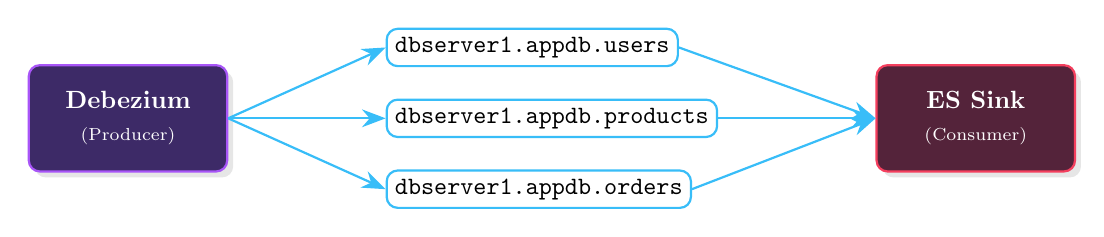
\begin{tikzpicture}[node distance=1.5cm, every node/.style={scale=0.9}]
      \node[component, fill=cDebezium!30!surface, draw=cDebezium] (prod) {\textbf{Debezium}\\[0.1em]\scriptsize (Producer)};
      
      \node[rectangle, draw=accent, thick, rounded corners, right=2cm of prod, yshift=1cm] (t1) {\texttt{dbserver1.appdb.users}};
      \node[rectangle, draw=accent, thick, rounded corners, right=2cm of prod] (t2) {\texttt{dbserver1.appdb.products}};
      \node[rectangle, draw=accent, thick, rounded corners, right=2cm of prod, yshift=-1cm] (t3) {\texttt{dbserver1.appdb.orders}};
      
      \node[component, fill=cElastic!30!surface, draw=cElastic, right=2cm of t2] (cons) {\textbf{ES Sink}\\[0.1em]\scriptsize (Consumer)};

      \draw[arrow] (prod.east) -- (t1.west);
      \draw[arrow] (prod.east) -- (t2.west);
      \draw[arrow] (prod.east) -- (t3.west);
      
      \draw[arrow] (t1.east) -- (cons.west);
      \draw[arrow] (t2.east) -- (cons.west);
      \draw[arrow] (t3.east) -- (cons.west);
    \end{tikzpicture}
  \end{center}

  \vspace{0.2cm}
  \begin{center}
    \footnotesize
    \begin{tabular}{@{}lllc@{}}
      \toprule
      \textbf{Topic Name} & \textbf{Partitions} & \textbf{Retention} & \textbf{Message Key} \\
      \midrule
      \texttt{dbserver1.appdb.users} & 1 (Order guaranteed) & 7 days & MongoDB \texttt{\_id} \\
      \texttt{dbserver1.appdb.products} & 1 (Order guaranteed) & 7 days & MongoDB \texttt{\_id} \\
      \texttt{dbserver1.appdb.orders} & 1 (Order guaranteed) & 7 days & MongoDB \texttt{\_id} \\
      \bottomrule
    \end{tabular}
  \end{center}

  \vspace{0.2cm}
  % PLACEHOLDER: replace with actual screenshot
  \imageplaceholder{kafka-ui.png}{0.7\textwidth}{1.5cm}
  \vspace{-0.3cm}
  \begin{center}\scriptsize\color{textsec} Kafka UI showing live topic throughput\end{center}
\end{frame}

% ==================================================================
% SLIDE 13: ELASTICSEARCH: THE DESTINATION
% ==================================================================
\begin{frame}[fragile]{Elasticsearch: The Destination}
  \begin{columns}[T]
    \begin{column}{0.4\textwidth}
      \vspace{0.5cm}
      \begin{itemize}
        \item \textbf{Upsert Method:} If ID exists $\rightarrow$ update. If not $\rightarrow$ insert.
        \item \textbf{Regex Router SMT:} Strips the ugly \texttt{dbserver1.appdb.} prefix so indices are cleanly named.
        \item \textbf{Tombstone Handling:} Deletes documents natively when Debezium sends a null payload.
        \item \textbf{ID Mapping:} Forces ES to use the exact MongoDB \texttt{\_id}.
      \end{itemize}
    \end{column}
    \begin{column}{0.55\textwidth}
      \begin{tcolorbox}[codebox]
\begin{minted}{json}
{
  "name": "elasticsearch-sink",
  "config": {
    "connector.class": "io.aiven...ElasticsearchSinkConnector",
    "topics": "dbserver1.appdb.users",
    "write.method": "upsert",
    "key.ignore": "false",
    "behavior.on.null.values": "delete",
    "transforms": "extractId,renameTopics,removeId",
    "transforms.renameTopics.type": "...RegexRouter",
    "transforms.renameTopics.regex": "dbserver1\\.appdb\\.(.*)",
    "transforms.renameTopics.replacement": "$1"
  }
}
\end{minted}
      \end{tcolorbox}
    \end{column}
  \end{columns}

  \vspace{0.3cm}
  % PLACEHOLDER: replace with actual screenshot
  \imageplaceholder{kibana-discover.png}{0.45\textwidth}{1.5cm}
  \vspace{-0.3cm}
  \begin{center}\scriptsize\color{textsec} Kibana Discover showing real-time indexed documents\end{center}
\end{frame}

% ==================================================================
% SLIDE 14: SECTION DIVIDER 3
% ==================================================================
\begin{frame}[plain]
  \begin{tikzpicture}[remember picture, overlay]
    \fill[bgbody] (current page.south west) rectangle (current page.north east);
    \fill[accent] (current page.south west) rectangle ([xshift=0.33\paperwidth]current page.north west);
    
    \begin{scope}[opacity=0.2]
      \draw[white, thick] (-1,0) -- (4,5);
      \draw[white, thick] (-1,2) -- (4,7);
      \draw[white, thick] (-1,4) -- (4,9);
    \end{scope}

    \node[anchor=center, text=primary, font=\fontsize{60}{60}\bfseries] at ([xshift=0.165\paperwidth]current page.center) {03};
    
    \node[anchor=west, text=white] at ([xshift=0.38\paperwidth]current page.west) {
      \begin{minipage}{0.55\textwidth}
        {\Huge\bfseries Live Pipeline Demo}\\[0.5em]
        {\Large\color{accentsec} Sub-200ms from write to search.}
      \end{minipage}
    };
  \end{tikzpicture}
\end{frame}

% ==================================================================
% SLIDE 15: DEMO LIFECYCLE
% ==================================================================
\begin{frame}{Demo: Step-by-Step Event Lifecycle}
  \begin{columns}
    \begin{column}{0.65\textwidth}
      \begin{tikzpicture}[node distance=0.8cm, auto]
        \draw[accentsec, thick] (0,-0.5) -- (0,-5.5);
        
        \node[stepcircle] (s1) at (0,0) {1};
        \node[right=0.3cm of s1, text=white] {\textbf{App inserts document} \small \textcolor{textsec}{\faArrowRight\ MongoDB}};

        \node[stepcircle] (s2) at (0,-1.2) {2};
        \node[right=0.3cm of s2, text=white] {\textbf{MongoDB engine writes to oplog}};

        \node[stepcircle] (s3) at (0,-2.4) {3};
        \node[right=0.3cm of s3, text=white] {\textbf{Debezium tailer detects oplog entry}};

        \node[stepcircle] (s4) at (0,-3.6) {4};
        \node[right=0.3cm of s4, text=white] {\textbf{Event published to Kafka topic}};

        \node[stepcircle] (s5) at (0,-4.8) {5};
        \node[right=0.3cm of s5, text=white] {\textbf{ES Sink consumes event \& Upserts}};

        \node[stepcircle] (s6) at (0,-6.0) {6};
        \node[right=0.3cm of s6, text=white] {\textbf{Document instantly searchable in Elastic}};
      \end{tikzpicture}
    \end{column}
    \begin{column}{0.35\textwidth}
      \begin{tcolorbox}[card, colback=accent!10!surface, colframe=accent, boxrule=1pt, halign=center]
        \Huge \textbf{\textcolor{accent}{\textasciitilde50ms}}\\
        \normalsize \textcolor{textsec}{End-to-End Latency}
      \end{tcolorbox}
      
      \vspace{0.5cm}
      % PLACEHOLDER: replace with actual screenshot
      \imageplaceholder{demo-terminal.png}{\textwidth}{3cm}
      \vspace{-0.3cm}
      \begin{center}\scriptsize\color{textsec} Terminal output during live demo\end{center}
    \end{column}
  \end{columns}
\end{frame}

% ==================================================================
% SLIDE 16: PYTHON DEMO APPLICATION
% ==================================================================
\begin{frame}[fragile]{Demo: Python Application Output}
  \begin{columns}[T]
    \begin{column}{0.48\textwidth}
      \begin{tcolorbox}[codebox]
\begin{minted}{python}
while True:
  # 1. Insert into MongoDB
  doc_id, _ = do_insert(collection)
  
  # 2. Wait briefly
  time.sleep(0.5)
  
  # 3. Query Elasticsearch directly
  es_state = query_es(session, doc_id)
  
  # 4. Measure latency & print
  latency_ms = (t_end - t_start) * 1000
  print_comparison(doc_id, es_state, latency_ms)
\end{minted}
      \end{tcolorbox}
    \end{column}
    \begin{column}{0.48\textwidth}
      \begin{tcolorbox}[card, colback=black, colframe=black, coltext=green!80!white, fontupper=\ttfamily\scriptsize]
[INSERT] user\_id=abc123 \faArrowRight\ MongoDB: OK\\
[QUERY]  user\_id=abc123 \faArrowRight\ Elasticsearch:\\
\hspace*{1cm} FOUND (lag: 42.1ms)\\
----------------------------------------\\
[UPDATE] user\_id=abc123 \faArrowRight\ MongoDB: OK\\
[QUERY]  user\_id=abc123 \faArrowRight\ Elasticsearch:\\
\hspace*{1cm} UPDATED (lag: 53.8ms)\\
----------------------------------------\\
[DELETE] user\_id=abc123 \faArrowRight\ MongoDB: OK\\
[QUERY]  user\_id=abc123 \faArrowRight\ Elasticsearch:\\
\hspace*{1cm} NOT FOUND (lag: 39.4ms)
      \end{tcolorbox}
    \end{column}
  \end{columns}
  
  \vspace{0.4cm}
  % PLACEHOLDER: replace with actual screenshot
  \imageplaceholder{demo-output.png}{0.5\textwidth}{1.5cm}
\end{frame}

% ==================================================================
% SLIDE 17: SECTION DIVIDER 4
% ==================================================================
\begin{frame}[plain]
  \begin{tikzpicture}[remember picture, overlay]
    \fill[bgbody] (current page.south west) rectangle (current page.north east);
    \fill[accent] (current page.south west) rectangle ([xshift=0.33\paperwidth]current page.north west);
    
    \begin{scope}[opacity=0.2]
      \draw[white, thick] (-1,0) -- (4,5);
      \draw[white, thick] (-1,2) -- (4,7);
      \draw[white, thick] (-1,4) -- (4,9);
    \end{scope}

    \node[anchor=center, text=primary, font=\fontsize{60}{60}\bfseries] at ([xshift=0.165\paperwidth]current page.center) {04};
    
    \node[anchor=west, text=white] at ([xshift=0.38\paperwidth]current page.west) {
      \begin{minipage}{0.55\textwidth}
        {\Huge\bfseries Results \& Observability}\\[0.5em]
        {\Large\color{accentsec} Ensuring reliability in production.}
      \end{minipage}
    };
  \end{tikzpicture}
\end{frame}

% ==================================================================
% SLIDE 18: PERFORMANCE RESULTS
% ==================================================================
\begin{frame}{Performance Results}
  \begin{columns}
    \begin{column}{0.31\textwidth}
      \begin{tcolorbox}[card, colframe=accent, boxrule=1pt, halign=center]
        \Large \textbf{\textcolor{accent}{< 200ms}}\\ \scriptsize Average Latency
      \end{tcolorbox}
    \end{column}
    \begin{column}{0.31\textwidth}
      \begin{tcolorbox}[card, colframe=success, boxrule=1pt, halign=center]
        \Large \textbf{\textcolor{success}{100\%}}\\ \scriptsize Delivery Guarantee
      \end{tcolorbox}
    \end{column}
    \begin{column}{0.31\textwidth}
      \begin{tcolorbox}[card, colframe=accentsec, boxrule=1pt, halign=center]
        \Large \textbf{\textcolor{accentsec}{0}}\\ \scriptsize Docs Lost on Restart
      \end{tcolorbox}
    \end{column}
  \end{columns}

  \vspace{0.4cm}
  \begin{columns}
    \begin{column}{0.45\textwidth}
      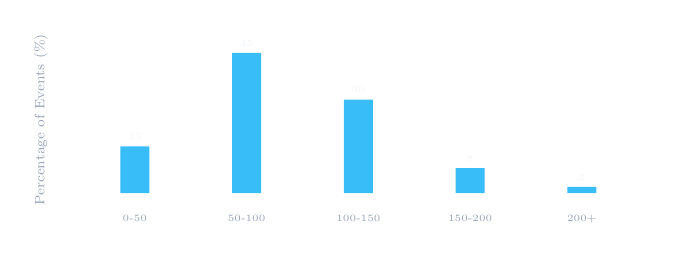
\begin{tikzpicture}[scale=0.7]
        \begin{axis}[
            ybar,
            bar width=15pt,
            width=\textwidth,
            height=4.5cm,
            enlarge x limits=0.15,
            ylabel={Percentage of Events (\%)},
            symbolic x coords={0-50, 50-100, 100-150, 150-200, 200+},
            xtick=data,
            nodes near coords,
            nodes near coords align={vertical},
            every node near coord/.append style={font=\tiny, color=textprim},
            axis line style={draw=none},
            tick style={draw=none},
            yticklabels={,,},
            x tick label style={font=\tiny, text=textsec},
            y tick label style={font=\tiny, text=textsec},
            ylabel style={font=\scriptsize, text=textsec}
        ]
        \addplot[fill=accent, draw=none] coordinates {
          (0-50, 15) (50-100, 45) (100-150, 30) (150-200, 8) (200+, 2)
        };
        \end{axis}
      \end{tikzpicture}
    \end{column}
    \begin{column}{0.5\textwidth}
      % PLACEHOLDER: replace with actual screenshot
      \imageplaceholder{grafana-dashboard.png}{\textwidth}{3cm}
      \vspace{-0.3cm}
      \begin{center}\scriptsize\color{textsec} Grafana dashboard — consumer lag near zero\end{center}
    \end{column}
  \end{columns}
\end{frame}

% ==================================================================
% SLIDE 19: MONITORING STACK
% ==================================================================
\begin{frame}{Monitoring Stack}
  \begin{columns}
    \begin{column}{0.48\textwidth}
      \begin{tcolorbox}[card, title=\faStream\ Kafka UI (Port 8080)]
        \scriptsize Browse topics, inspect live JSON messages, and track consumer group lag natively.
      \end{tcolorbox}
      \begin{tcolorbox}[card, title=\faChartArea\ Prometheus (Port 9090)]
        \scriptsize Scrape JMX metrics directly from Kafka brokers and Debezium worker nodes.
      \end{tcolorbox}
    \end{column}
    \begin{column}{0.48\textwidth}
      \begin{tcolorbox}[card, title=\faChartBar\ Grafana (Port 3000)]
        \scriptsize Dashboards for throughput, network latency, partition health, and error rates.
      \end{tcolorbox}
      \begin{tcolorbox}[card, title=\faSearch\ Kibana (Port 5601)]
        \scriptsize Run complex queries and visually verify indexed documents and data schemas.
      \end{tcolorbox}
    \end{column}
  \end{columns}

  \vspace{0.4cm}
  % PLACEHOLDER: replace with actual screenshot
  \imageplaceholder{monitoring-overview.png}{0.65\textwidth}{2.5cm}
\end{frame}

% ==================================================================
% SLIDE 20: SECTION DIVIDER 5
% ==================================================================
\begin{frame}[plain]
  \begin{tikzpicture}[remember picture, overlay]
    \fill[bgbody] (current page.south west) rectangle (current page.north east);
    \fill[accent] (current page.south west) rectangle ([xshift=0.33\paperwidth]current page.north west);
    
    \begin{scope}[opacity=0.2]
      \draw[white, thick] (-1,0) -- (4,5);
      \draw[white, thick] (-1,2) -- (4,7);
      \draw[white, thick] (-1,4) -- (4,9);
    \end{scope}

    \node[anchor=center, text=primary, font=\fontsize{60}{60}\bfseries] at ([xshift=0.165\paperwidth]current page.center) {05};
    
    \node[anchor=west, text=white] at ([xshift=0.38\paperwidth]current page.west) {
      \begin{minipage}{0.55\textwidth}
        {\Huge\bfseries Key Takeaways}\\[0.5em]
        {\Large\color{accentsec} Why this architecture matters.}
      \end{minipage}
    };
  \end{tikzpicture}
\end{frame}

% ==================================================================
% SLIDE 21: KEY TAKEAWAYS
% ==================================================================
\begin{frame}{Key Takeaways}
  \vspace{0.5cm}
  \begin{itemize}
    \item[\textcolor{accent}{\textbf{1.}}] \textbf{Eliminates Batching:} Changes propagate in real time, not overnight.
    \vspace{0.2cm}
    \item[\textcolor{accent}{\textbf{2.}}] \textbf{Zero App Changes:} Debezium reads the oplog entirely invisibly.
    \vspace{0.2cm}
    \item[\textcolor{accent}{\textbf{3.}}] \textbf{Decoupled Arch:} Kafka isolates MongoDB performance from Elasticsearch indexing.
    \vspace{0.2cm}
    \item[\textcolor{accent}{\textbf{4.}}] \textbf{KRaft is the Future:} Zookeeper removal simplifies Ops significantly.
    \vspace{0.2cm}
    \item[\textcolor{accent}{\textbf{5.}}] \textbf{Highly Portable:} The entire clustered stack runs flawlessly in Docker.
  \end{itemize}

  \vspace{0.8cm}
  \begin{center}
    % PLACEHOLDER: replace with actual logos
    \imageplaceholder{logo-mongo.png}{2cm}{1cm} \quad
    \imageplaceholder{logo-debezium.png}{2cm}{1cm} \quad
    \imageplaceholder{logo-kafka.png}{2cm}{1cm} \quad
    \imageplaceholder{logo-elasticsearch.png}{2cm}{1cm}
  \end{center}
\end{frame}

% ==================================================================
% SLIDE 22: THANK YOU / Q&A
% ==================================================================
\begin{frame}[plain]
  \begin{center}
    \vspace{1cm}
    {\Huge\bfseries\color{accent} Thank You!}\\[0.5em]
    {\Large\color{textprim} Any Questions?}
    \vspace{1cm}

    \begin{columns}
      \begin{column}{0.31\textwidth}
        \begin{tcolorbox}[card, halign=center, size=small]
          \textcolor{textsec}{\faGithub\ GitHub}\\[0.2em]
          \scriptsize \href{https://github.com/repo}{github.com/repo}
        \end{tcolorbox}
      \end{column}
      \begin{column}{0.31\textwidth}
        \begin{tcolorbox}[card, halign=center, size=small]
          \textcolor{textsec}{\faLinkedin\ LinkedIn}\\[0.2em]
          \scriptsize \href{https://linkedin.com/in/user}{linkedin.com/in/user}
        \end{tcolorbox}
      \end{column}
      \begin{column}{0.31\textwidth}
        \begin{tcolorbox}[card, halign=center, size=small]
          \textcolor{textsec}{\faEnvelope\ Email}\\[0.2em]
          \scriptsize \href{mailto:email@example.com}{email@example.com}
        \end{tcolorbox}
      \end{column}
    \end{columns}

    \vspace{0.8cm}
    % PLACEHOLDER: replace with actual screenshot
    \imageplaceholder{qr-code.png}{2cm}{2cm}
    \vspace{-0.3cm}
    \begin{center}\scriptsize\color{textsec} Scan for the full source code\end{center}
  \end{center}
\end{frame}

\end{document}
